\documentclass[12pt,a4paper,french]{report}
\usepackage[utf8]{inputenc}
\usepackage[T1]{fontenc}
\usepackage[french]{babel}
\usepackage{graphicx}
\usepackage{amsmath}
\usepackage{amssymb}
\usepackage{geometry}
\usepackage{fancyhdr}
\usepackage{hyperref}
\hypersetup{
	colorlinks=true,
	linkcolor=blue,
	citecolor=blue,
	urlcolor=blue,
	bookmarksnumbered=true
}
\usepackage{booktabs}
\usepackage{float}
\usepackage{caption}
\usepackage{subcaption}
\usepackage{array}
\usepackage{xcolor}
\usepackage{listings}
\usepackage[backend=biber, style=authoryear, sorting=none, doi=true, url=true, isbn=false]{biblatex}
\addbibresource{references.bib}

% Configuration de la géométrie
\geometry{
	top=2.5cm,
	bottom=2.5cm,
	left=2.5cm,
	right=2.5cm
}

% Configuration des en-têtes et pieds de page
\pagestyle{fancy}
\fancyhf{}
\rhead{\thepage}
\lhead{\leftmark}
\renewcommand{\headrulewidth}{0.4pt}

% Configuration des titres
\usepackage{titlesec}
\titleformat{\chapter}[display]
{\normalfont\Large\bfseries}
{\chaptertitlename\ \thechapter}{20pt}{\Large}
\titlespacing*{\chapter}{0pt}{50pt}{40pt}

\title{Modélisation du fret routier au Rwanda \\[0.5em]
	\large Mémoire de master EEET, parcours modélisation prospective}
\author{DUMAS Yanis}
\date{8 septembre 2026}

\begin{document}
	
	\maketitle
	
	\newpage
	
	% Table des matières
	\tableofcontents
	\newpage
	
	% Remerciements
	\chapter*{Remerciements}
	\addcontentsline{toc}{chapter}{Remerciements}
	
	[À remplir]
	
	\newpage
	
	% Introduction
	\chapter{Introduction}
	
	En 2021 sortait le dernier rapport du GIEC \cite{IPCC2021} sur les bases physiques du dérèglement climatique. De manière très classique, il est rappelé que ce dernier implique une augmentation de la fréquence et de l'intensité des événements climatiques extrêmes, notamment des inondations, à travers le monde.
	
	\begin{figure}[H]
		\centering
		\begin{minipage}{0.48\textwidth}
			\centering
			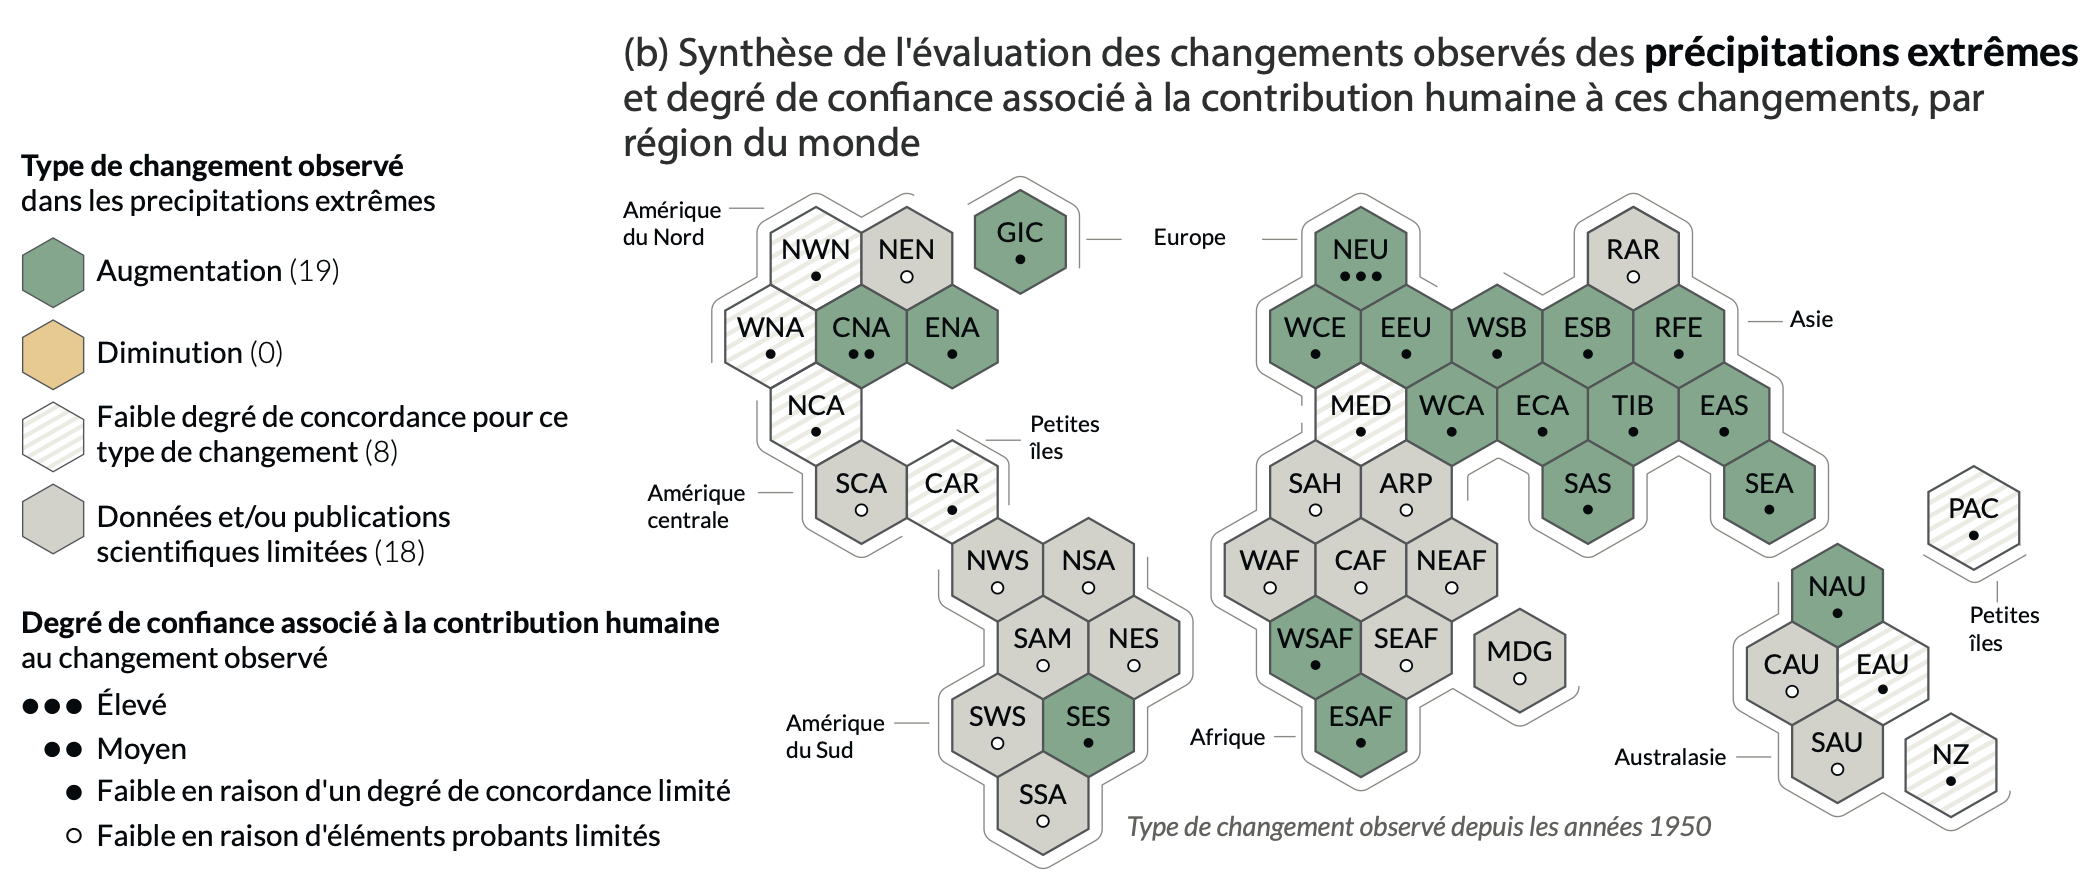
\includegraphics[width=\linewidth]{images/evol_hist_precip.png}
			\caption{Évolution historique des précipitations extrêmes\\
				\footnotesize Source : \cite{IPCC2021}}
			\label{fig:frequence}
		\end{minipage}
		\hfill
		\begin{minipage}{0.35\textwidth}
			\centering
			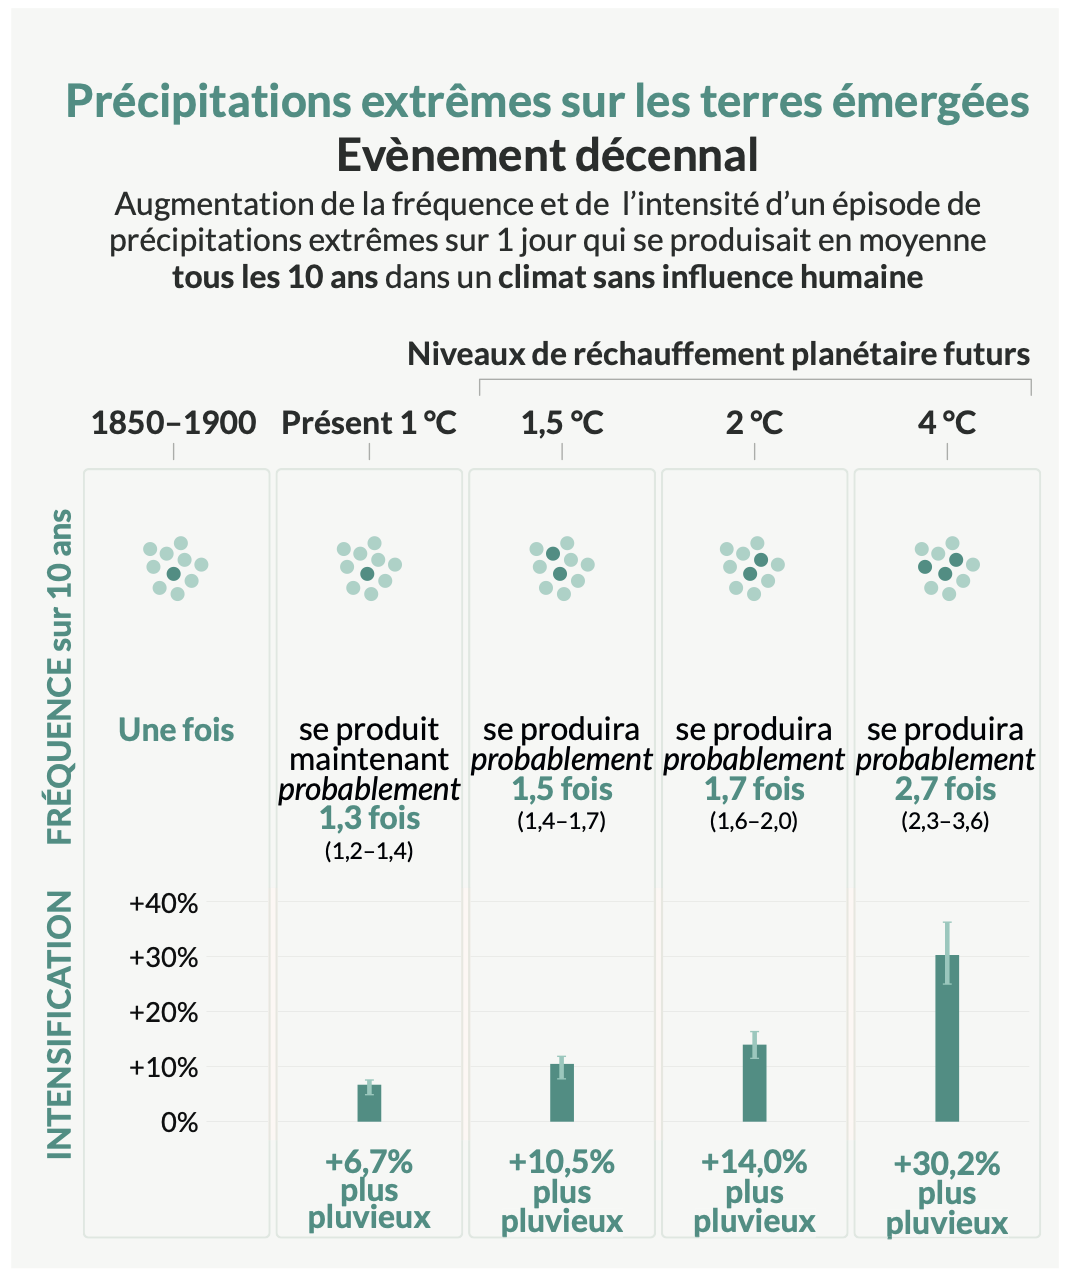
\includegraphics[width=\linewidth]{images/evol_prevue_precip.png}
			\caption{Projection de l'évolution des précipitations extrêmes \\
				\footnotesize Source : \cite{IPCC2021}}
			\label{fig:giec}
		\end{minipage}
	\end{figure}
	
	Ces événements extrêmes ont des conséquences importantes sur les infrastructures, notamment de transport. Or, les réseaux de transport ont une place très centrale dans l'organisation des chaînes de valeur. Le transport est un service de base au sens de P. Sraffa, c'est-à-dire qu'il intervient dans la formation des prix de l'ensemble des biens et services de l'économie. D'autre part, le transport est à la base de la division nationale et internationale du travail permettant de réaliser de fort gain d'efficacité. Ainsi, un choc sur ce dernier peut se diffuser à l'ensemble de l'économie et avoir une effet important sur l'inflation et/ou sur la production agrégées. Ainsi, si l'on veut faire une analyse fine de la vulnérabilité des économies nationales aux catastrophes naturelles, il est nécessaire de modéliser explicitement le secteur des transports.
	
	D'autre part, les catastrophes naturelles sont des événements ponctuels, de court terme et souvent localisés. De ce fait, il est important d'adopter une approche spatialement explicite et sectorielle afin d'avoir une meilleure compréhension de la diversité de ses impacts. C'est cela l'objectif de ce mémoire, présenter la construction d'un modèle de transport de fret spatialisé couplable avec un modèle macroéconomique de court-terme multisectoriel.
	
	\newpage
	
	% Revue de littérature
	\chapter{Revue de littérature}
	
	Il existe aujourd'hui un nombre important de manière de modéliser le fret. Ces différentes méthodes ont toutes des avantages et des inconvénients. Nous allons essayer d'en faire une rapide revue.
	
	\section {Les types de modèles de fret}
	\label{sec:type_modele}
	
	\subsection {SCGE}
	\label{subsec:SCGE}
	
	Une façon possible de représenter le fret, qui aurait l'avantage d'être directement connecté à un modèle macroéconomique multisectoriel, est d'utiliser un Spatial Computable General Equilibrium (SCGE). Dans ce type de modèle, les volumes d'échanges, calibrés sur les données des tables Input-Output (IO), sont endogènes et varient en fonction des prix. Le territoire représenté est divisé en plusieurs sous-territoire avec leur propre décomposition IO. Ces différents sous-territoires échanges entre eux sous la forme d'un commerce extérieur. Le fret est ici ou bien un secteur comme un autre utilisé comme consommation intermédiaire, ou bien directement un coût exogène a intégré dans le prix des autres secteurs. Le principale problème de ce type de modélisation pour notre sujet est qu'il n'intègre pas explicitement le réseau de transport. Un choc comme une innondation détruisant des infrastructures de transport est modélisé uniquement via un surcoût agrégé du secteur du fret. L'emplacement du choc n'a donc pas vraiment d'importance.
	
	\subsection {Agregate, Desagregate, Agregate (ADA)}
	\label{subsec:ADA}
	
	Dans ce type de modélisation, le réseau de transport est très important et très détaillé. Les modèles ADA représentent explicitement l'ensemble des étapes de la chaine logistique (embarquement, passage par un hub de distribution, manutention, stockage, etc...). Ils permettent d'endogénéisé de manière précise et conjointe la taille des envoies (c'est-à-dire le volume de marchandises par véhicule), le mode de transport utilisé et le chemin précis empreinté sur le réseau. 
	
	\subsection {Agent-Based Model (ABM) ou microsimulations}
	\label{subsec:ABM}
		
	La spécificité de ce type de modèle, qui fait à la fois sa force et sa faiblesse, est que son objectif premier est de modéliser les flux à l'échelle de l'agent. Chaque firme individuelle est représentée et interagit avec les autres firmes modélisés. Il n'y a pas de firme représentative (ou à un niveau particulièrement désagrégé) ni de bouclage macroéconomique forcé. La dynamique d'ensemble émerge des comportements individuels tel que modélisés. Un choc est là aussi modélisé par la coupure d'un arc du réseau. Les mécanismes de diffusion de ce choc peuvent ainsi être représenté de manière particulièrement fine. Le principal problème de ce type de modèle c'est qu'ils sont particulièrement complexe à calibré et nécessite de surcroît une quantité de données particulièrement massive.
	
	\subsection {Modèles de machine learning}
	\label{subsec:machine_learning}
	
	Ces modèles sont beaucoup utilisé pour de la prospective, notamment par des entreprises privées comme Amazon par exemple. L'avantage de ce type d'approche c'est qu'elle nécessite une nombre minimal de choix de forme fonctionnelle mais nécessite en contrepartie un nombre encore plus important que pour les ABM de données.
	
	\section{Le modèle classique à 4 étapes}
	\label{sec:4_etapes}
	
	Le type de modèle le plus fréquent pour représenter le fret, d'après \cite{deJong2004}, que nous avons décider d'utiliser dans ce projet est la structure en 4 étapes.  Cette dernière est inspirée très largement des modèles du même nom concernant le transport de personnes. Elle se décompose, comme son nom l'indique, en 4 étapes : production et attraction, choix des destinations, choix du mode de transport et choix de la route empruntée. Chacune de ces étapes peut être modélisée selon plusieurs méthodes. Nous nous appuierons, dans cette partie, largement sur la revue de \cite{deJong2004}. Ce type de modèle à l'avantage d'une plus grande simplicité dans son principe de base, d'avoir été particulièrement éprouvé dans la littérature et de permettre d'incorporer progressivement certain avantage des autres approches méthodologiques comme la prise en compte d'une diversité de coûts du réseau ainsi l'usage de données IO, facilitant le couplage ultérieur avec un modèle multisectoriel. 
	
	\subsection{Production et attraction}
	\label{subsec:prod_attraction}
	
	Cette étape consiste à attribuer aux différents points censés échanger entre eux la quantité de marchandises sortant et entrant de ces derniers. Ces points sont les origines et destinations des véhicules modélisés. \cite{deJong2004} distinguent quatre familles de méthodes pour déterminer ces volumes, toutes construites, à la date de leur revue, à partir de données agrégées. Nous les présentons successivement en associant à chacune une référence théorique ou de revue et une application publiée, avant d'expliciter celle que nous retenons.

	\paragraph{Séries temporelles.} La première famille consiste à extrapoler des séries de trafic observé, éventuellement ventilées par type de marchandises, à l'aide de modèles économétriques temporels. \cite{Meersman2013} en proposent la discussion théorique de référence : ils examinent la relation entre activité économique et volumes de fret et montrent que le recours au PIB agrégé comme unique variable explicative est un mauvais prédicteur, parce qu'il masque les changements de composition sectorielle et de comportement logistique des chargeurs ; ils plaident pour des approches plus désagrégées. Une application caractéristique est fournie par \cite{Rashed2017}, qui prévoient à court terme le trafic conteneurisé mensuel du port d'Anvers au moyen d'un modèle ARIMA à interventions estimé sur la période 1995--2015. Ce type d'approche prolonge les tendances historiques sans faire intervenir de facteurs explicatifs extérieurs à la série elle-même. Elle suppose donc de disposer de longues séries de trafic observé — ce dont nous ne disposons pas au Rwanda (section~\ref{sec:contexte_modele}) — et ne dit rien de la localisation de la demande. Elle n'est donc pas utilisable ici.

	\paragraph{Systèmes dynamiques.} La deuxième famille représente l'économie et le transport comme un ensemble de stocks, de flux et de boucles de rétroaction simulés dans le temps, selon le cadre formalisé par \cite{Sterman2000}. L'application la plus aboutie dans le champ du transport est le modèle européen ASTRA \cite{Fiorello2010} : construit sous Vensim, il articule neuf modules reliant croissance économique, demande de transport, parc de véhicules et effets environnementaux, et sert à l'évaluation stratégique de politiques européennes de long terme. L'intérêt de cette famille est double : le bouclage macroéconomique est explicite et la dimension temporelle est traitée nativement, ce qui est précieux pour un couplage. Sa limite pour notre objet est que, comme le reconnaissent \cite{Fiorello2010}, ASTRA est nettement moins détaillé géographiquement qu'un modèle de transport classique : le réseau n'y est pas représenté arc par arc, et un choc localisé sur une route ne peut donc pas y être modélisé.

	\paragraph{Taux de génération par zone.} La troisième famille estime économétriquement, pour chaque zone, un volume produit ou attiré en fonction de variables observables (emploi, surface d'activité, population, secteur). \cite{SanchezDiaz2016} en donnent une application représentative en estimant des modèles d'attraction de déplacements de fret intégrant explicitement les effets spatiaux entre zones voisines. Sur le plan théorique, \cite{HolguinVeras2011} constituent la référence critique : ils établissent qu'il faut distinguer la \emph{génération de fret} (en tonnes, déterminée par l'économie de la production et de la consommation) de la \emph{génération de déplacements de fret} (en véhicules, qui résulte de décisions logistiques), et montrent que l'usage de taux de génération constants par zone est d'autant plus biaisé que les établissements sont hétérogènes et que l'agrégation spatiale est grossière. Cet avertissement vaut directement pour notre modèle : il justifie que nous spatialisions des tonnes, et que le passage aux véhicules soit traité séparément, au stade de l'affectation (section~\ref{subsubsec:PCU}).

	\paragraph{Tables entrée-sortie.} La dernière famille dérive les volumes échangés de la structure entrée-sortie de l'économie : la production sectorielle d'une zone engendre, via les coefficients techniques, une demande d'intrants qui doit être satisfaite quelque part. \cite{Miller2009} en fournissent le cadre théorique complet (comptabilité entrée-sortie, inverse de Leontief, extensions multirégionales). \cite{Cascetta2008} en donnent l'application de référence en modélisation du fret : ils construisent un modèle entrée-sortie multirégional simulant, à l'échelle nationale italienne, à la fois la génération et la distribution spatiale des flux de marchandises, articulé en aval avec des modèles de choix modal et d'itinéraire. C'est cette quatrième voie que nous retenons (section~\ref{subsubsec:affectation_prod}), pour deux raisons : elle est la seule à garantir la cohérence comptable entre les flux physiques modélisés et les grandeurs macroéconomiques, et elle est la seule à rendre le modèle directement couplable avec un modèle multisectoriel, ce qui est l'objectif final du travail.
	
	\subsection{Distribution}
	\label{subsec:distrib}
	
	L'objectif de cette étape est de déterminer les volumes de transport entre chacune des origines et destinations $(f_{i,j})$. Le modèle le plus utilisé est le modèle gravitaire. L'intuition de ce modèle est que deux zones ont d'autant plus de chance d'échanger entre elles qu'elles sont de grande taille et que le coût de transport entre les deux points est faible.

	Sur le plan théorique, ce modèle ne relève pas seulement de l'analogie physique. \cite{Wilson1967} lui donne son fondement le plus utilisé en modélisation des transports : la matrice gravitaire est la distribution la plus probable, c'est-à-dire celle qui maximise l'entropie, parmi toutes les matrices compatibles avec les marges d'émission et d'attraction et avec un budget de coût de transport donné. Les facteurs d'équilibrage $A_i$ et $B_j$ y apparaissent comme les multiplicateurs de Lagrange des contraintes de marge, et le paramètre $\beta$ de la fonction de découragement comme celui de la contrainte de coût. \cite{Anderson2003} en fournissent le pendant du côté du commerce international, en montrant qu'une équation gravitaire structurelle se dérive d'un modèle d'équilibre général avec préférences CES, et que les flux bilatéraux dépendent non du coût bilatéral absolu mais de son rapport aux « résistances multilatérales » de chaque zone — l'analogue économique exact des facteurs d'équilibrage de Wilson.

	Du côté des applications, \cite{Cai2021} est particulièrement proche de notre usage : il montre que plusieurs procédures d'estimation de matrices de commerce interrégional documentées dans la littérature se ramènent en réalité à un même modèle gravitaire doublement contraint, que ce modèle exige beaucoup moins de données qu'on ne le suppose généralement, et que sous des hypothèses raisonnables les flux inconnus se retrouvent exactement par l'algorithme RAS — c'est-à-dire l'algorithme de Furness que nous employons (section~\ref{subsubsec:furness}). C'est un argument central pour notre travail : dans un contexte où aucune matrice origine-destination de fret n'est observée, le modèle gravitaire doublement contraint est précisément la méthode conçue pour reconstruire des flux à partir des seules marges et d'une mesure de coût.

	Nous développerons plus en détail cette méthode lors de la présentation du modèle utilisé dans le cadre de cette étude (section~\ref{subsubsec:gravitaire}).

	\subsection{Choix modale}
	\label{subsec:choix_modale}

	Cette étape répartit la demande totale de transport entre les modes disponibles (route, rail, voie d'eau, etc.). Le cadre théorique dominant est celui des modèles de choix discret : \cite{McFadden1974} montre que si l'utilité que le décideur associe à chaque alternative se décompose en une partie observable et un aléa de loi de Gumbel indépendant, la probabilité de choix prend la forme logit fermée. Chaque mode est alors caractérisé par un coût généralisé — prix, temps, fiabilité, coût de rupture de charge — et la répartition modale découle des écarts entre ces coûts. \cite{Tavasszy2014} en proposent la synthèse appliquée au fret, en soulignant la difficulté propre à ce champ : le décideur n'est pas un individu mais une chaîne d'acteurs (chargeur, commissionnaire, transporteur), et le choix du mode est indissociable du choix de la taille des envois.

	L'application de référence retenue ici est celle de \cite{Rich2009}, qui estiment un logit pondéré de choix conjoint du mode et du point de franchissement dans la région de l'Öresund, et en tirent des élasticités au coût monétaire et au temps ainsi que des valeurs du temps par mode et par groupe de marchandises. Ce travail illustre à la fois la puissance de l'approche et son exigence : elle suppose des données d'enquête chargeurs désagrégées, inexistantes dans notre cas.

	Dans le modèle présenté ici, cette étape est fortement contrainte par le contexte : l'absence de rail et de voie d'eau au Rwanda (section~\ref{sec:tout_routier}) réduit le choix modal à un choix de type de véhicule, traité de manière déterministe par minimisation du coût généralisé sur un graphe multimodal, donc conjointement avec l'étape d'assignation (section~\ref{subsubsec:cout_generalise}).

	\subsection{Assignation}
	\label{subsec:assignation}

	La dernière étape affecte les flux origine-destination aux arcs du réseau. Le principe théorique est celui du premier principe de \cite{Wardrop1952} : à l'équilibre, aucun usager ne peut réduire son coût en changeant unilatéralement d'itinéraire, de sorte que tous les itinéraires effectivement empruntés entre une même paire ont le même coût, inférieur ou égal à celui des itinéraires inutilisés. \cite{Beckmann1956} montrent que cet équilibre est la solution d'un programme d'optimisation convexe, ce qui en garantit l'existence et l'unicité en flux d'arcs ; \cite{Sheffi1985} en donne le traitement algorithmique de référence, dont la méthode des moyennes successives que nous utilisons (section~\ref{subsubsec:MSA}). La relation entre le flux d'un arc et son temps de parcours est le plus souvent décrite par la fonction débit-retard du \cite{BPR1964}, dont les paramètres standards $\alpha = 0{,}15$ et $\beta = 4$ sont encore ceux employés aujourd'hui.

	L'application la plus pertinente pour notre travail est le réseau virtuel de NODUS \cite{Jourquin1996}. Ces auteurs représentent l'ensemble des opérations de transport — chargement, déplacement, déchargement, transbordement, transit — comme autant d'arcs « virtuels » d'un graphe unique, sur lequel l'affectation se fait par simple minimisation d'un coût généralisé. L'intérêt méthodologique est direct : cette construction fusionne les étapes de choix modal et d'assignation en une seule, puisque le choix du mode devient un choix de chemin dans le graphe étendu. C'est exactement la structure que nous adoptons, avec des couches par type de véhicule reliées par des arêtes de transbordement (section~\ref{subsubsec:reseau_routier}).


	\newpage
	
	% Contextualisation du Rwanda
	\chapter{Contextualisation du Rwanda}
	\label{chap:contexte}

	Ce chapitre décrit les caractéristiques du Rwanda qui déterminent la géographie de son fret : la densité et le relief de son territoire, l'organisation de son système de transport, la structure de son appareil productif et son exposition aux aléas hydro-climatiques. Les conséquences de ce contexte sur la construction du modèle sont discutées au chapitre suivant (section~\ref{sec:contexte_modele}).

	\section{Un territoire dense et accidenté}
	\label{sec:territoire}

	Le cinquième recensement de la population et de l'habitat dénombre 13~246~394~habitants en août 2022, pour une croissance intercensitaire de 2,3~\% par an et une densité de 503~habitants par km$^2$, l'une des plus fortes d'Afrique continentale \cite{NISR2023}. Cette densité reste très largement rurale : la population urbaine ne représentait que 27,9~\% du total en 2022, contre 16,5~\% en 2012, et l'armature urbaine est nettement dominée par Kigali \cite{NISR2023}. L'activité économique et la population ne sont donc pas concentrées dans quelques pôles industriels, mais réparties sur un semis dense de collines habitées, ce qui conduit à des flux de marchandises nombreux, courts et diffus.

	Le relief accentue cette caractéristique. Le « pays aux mille collines » présente des dénivelés importants sur de courtes distances : la politique nationale des transports note que les tracés routiers suivent principalement les courbes de niveau, ce qui allonge sensiblement les distances parcourues par rapport à la distance à vol d'oiseau et dégrade l'efficacité du réseau \cite{MININFRA2021}. La pente affecte directement la consommation de carburant et la vitesse commerciale des poids lourds, et pèse d'autant plus que le véhicule est chargé.

	\section{Un système de transport entièrement routier}
	\label{sec:tout_routier}

	Le Rwanda ne dispose ni de réseau ferroviaire, ni de transport fluvial marchand d'ampleur, ni d'oléoduc en service. La politique nationale des transports est explicite : en l'absence de rail et de voies navigables, l'ensemble des marchandises entrant, sortant ou transitant par le pays est déplacé par camion \cite{MININFRA2021}. Les projets ferroviaires reliant Kigali aux ports de la région restent, à la date de rédaction, à l'état de planification. Le fret rwandais est donc, en pratique, un fret routier.

	Ce réseau routier est par ailleurs très hétérogène. Il comptait à la fin des années 2010 environ 44~671~km, dont seulement 1~973~km revêtus, 72~\% de ce linéaire bitumé correspondant aux routes nationales \cite{MININFRA2021}. Le fret longue distance se concentre donc sur une ossature bitumée étroite, tandis que l'essentiel du linéaire — routes de district et pistes de desserte — est en terre ou en latérite. Un tronçon revêtu interrompu n'a fréquemment pour report qu'une piste de qualité très inférieure.

	À cette structure interne s'ajoute la condition d'enclavement : le commerce maritime du pays transite par le territoire d'un pays tiers, principalement via le corridor Nord vers Mombasa (environ 1~682~km depuis Kigali) et le corridor Central vers Dar es Salaam (environ 1~495~km), auxquels s'ajoutent des échanges de proximité avec l'Ouganda, la Tanzanie, la RDC et le Burundi \cite{NCTTCA2018, MININFRA2021}. La politique nationale des transports qualifie le coût du transport, national comme international, d'« exceptionnellement élevé » et en fait une contrainte majeure au développement \cite{MININFRA2021}. Ce constat rejoint la littérature sur l'enclavement et les infrastructures \cite{Limao2001}, ainsi que les travaux de \cite{Storeygard2016} qui documentent, pour l'Afrique subsaharienne, l'effet des coûts de transport terrestre sur la géographie de l'activité, modulé par la qualité du revêtement des routes.

	\section{Une structure productive peu diversifiée}
	\label{sec:structure_productive}

	Malgré une croissance soutenue et une réduction rapide de la pauvreté depuis le milieu des années 1990, l'appareil productif rwandais reste marqué par le poids de l'agriculture dans l'emploi, un secteur manufacturier étroit et une croissance largement tirée par les services et l'investissement public \cite{WorldBank2020, WorldBank2024CEM}. Les biens manufacturés, les intrants industriels et les produits pétroliers sont pour l'essentiel importés, tandis que les exportations restent concentrées sur un petit nombre de produits (minerais, thé, café, réexportations) : le pays est structurellement importateur net dans la plupart des branches.

	Cette structure est décrite de façon cohérente par la matrice de comptabilité sociale (SAM) du Rwanda pour 2021, construite conjointement par l'IFPRI, le ministère des Finances et de la Planification économique (MINECOFIN) et l'Institut national des statistiques du Rwanda (NISR) dans le cadre du projet \emph{Nexus} \cite{IFPRI2023SAM}. Elle documente les coefficients techniques, la demande finale par secteur et par classe de ménage, la production nationale et le commerce extérieur sectoriel.

	\section{Une exposition marquée aux aléas hydro-climatiques}
	\label{sec:exposition_alea}

	La politique nationale des transports situe le Rwanda au 29\textsuperscript{e} rang mondial de vulnérabilité au changement climatique selon l'indice ND-GAIN, et identifie explicitement le risque de perturbation des systèmes de transport par les inondations, les vents violents et les glissements de terrain \cite{MININFRA2021}. La combinaison d'un relief accidenté, de fortes pluies saisonnières et d'une pression foncière élevée sur les versants rend les routes de montagne particulièrement exposées.

	L'épisode des 2 et 3~mai 2023 en fournit une illustration documentée. Des pluies torrentielles ont provoqué inondations et glissements de terrain dans les provinces de l'Ouest, du Nord et du Sud, causant plus de 130~décès. L'évaluation du MINECOFIN chiffre les dommages et pertes à 222,31~milliards de RWF (environ 193~millions d'USD) et les besoins de reconstruction à 518,58~milliards de RWF, pour un impact estimé à environ 0,4~point de croissance du PIB réel en 2023 \cite{MINECOFIN2023}. Surtout, \textbf{le secteur des transports concentre à lui seul près de 60~\% du total des dommages et pertes}, très loin devant le logement (12~\%), l'environnement et la gestion des ressources en eau (12~\%) et la santé (8~\%) \cite{MINECOFIN2023}. Au Rwanda, un aléa climatique localisé est donc d'abord un choc sur le réseau de transport.

	\newpage
	
	% Méthode utilisée
	\chapter{Méthode utilisée}
	
	\section{Orientation méthodologique générale}
	\label{sec:methodo_gene}
	
	Nous faisons ici un premier aperçu de la forme du modèle dont nous détaillerons plus précisément les parties dans le reste de ce mémoire.
	
	Le projet a été réalisé avec l'appui des différents modèles de LLM de l'entreprise Anthropic. Un abonnement payant à Claude Code de 20€/mois a été contracté pour faciliter le codage et débogage du modèle, la production de données fictives lorsque les données réelles manquaient, la revue de littérature et également pour aider à la réflexion sur les avantages et inconvénients des différents choix méthodologiques.
	
	Le projet reprend la structure des modèles en 4 étapes. Il se compose de la production d'un graphe multimodal représentant le réseau routier Rwandais. Sur chaque arc/arête de ce graphe, on applique une fonction de coût généralisé. Cette dernière est utilisée comme poids pour l'algorithme classique de plus court chemin (Dijkstra). Sur chaque nœud du graphe représentant les origines et destinations des flux, on alloue l'offre et la demande tel que définie dans la matrice de comptabilité sociale du Rwanda (c'est la partie production et attraction). Les flux d'échange sont ensuite modélisés à l'aide d'un modèle gravitaire (les étapes de distribution et de choix modal sont réalisées ici simultanément). De plus, on attribue les flux aux routes en tenant compte de la congestion (étape d'assignation). Enfin, nous produisons des scénarios de rupture des routes pour voir comment évolue le modèle dans ces cas.
	
	\section{Ce que le contexte rwandais impose au modèle}
	\label{sec:contexte_modele}

	Les caractéristiques décrites au chapitre~\ref{chap:contexte} ne sont pas de simples éléments de décor : elles contraignent directement la forme du modèle. Quatre d'entre elles sont structurantes.

	Premièrement, l'absence de rail et de voie d'eau réduit l'étape de choix modal du modèle à quatre étapes (section~\ref{subsec:choix_modale}) à un simple choix de \emph{type de véhicule} (camion lourd, camion léger, camionnette) : il n'existe pas d'arbitrage rail/route à représenter. La finesse du modèle se déporte donc entièrement sur la caractérisation des arcs routiers.

	Deuxièmement, l'hétérogénéité du réseau et le relief justifient un coût généralisé paramétré conjointement par type de véhicule, type de route et état de la route, plutôt que par une vitesse et une consommation moyennes (section~\ref{subsubsec:cout_generalise}). C'est également la raison pour laquelle un modèle numérique de terrain (Copernicus DEM) est mobilisé pour calculer la pente de chaque arc, à laquelle est associé un facteur de surconsommation spécifique à chaque type de véhicule.

	Troisièmement, le caractère diffus et rural de la population conduit à spatialiser l'offre et la demande à partir d'une grille de population fine (WorldPop, 100~m) agrégée par pavage de Voronoï autour des nœuds du graphe (sections~\ref{subsubsec:donnees_reelles} et~\ref{subsubsec:integ_donnees}), plutôt qu'à partir des seules unités administratives, qui masqueraient l'essentiel de la variabilité spatiale.

	Quatrièmement, le fait que le pays soit importateur net dans la plupart des branches a une conséquence technique directe sur l'équilibrage des flux : chercher à équilibrer par un algorithme de Furness un système où les surplus de production domestiques devraient couvrir à la fois la demande domestique et les exportations rend le problème infaisable pour les secteurs fortement déficitaires. C'est ce qui a conduit à décomposer le modèle gravitaire en trois jambes distinctes — domestique, export et import en brut — plutôt qu'à raisonner sur des soldes nets (section~\ref{subsubsec:decompo_comex}). Le commerce extérieur est par ailleurs représenté par une couche \emph{Rest of World} localisée aux postes frontières, assortie d'un coût pré-frontière par pays voisin (section~\ref{subsubsec:RoW}) ; il ne constitue toutefois pas l'objet central de la modélisation, qui porte avant tout sur les flux internes au territoire.

	Une dernière contrainte, d'ordre informationnel, doit être signalée. Si le contexte rwandais est bien documenté au niveau agrégé, les données de trafic de fret désagrégées (comptages routiers par tronçon, enquêtes chargeurs, matrices origine-destination observées) sont, à notre connaissance, indisponibles publiquement. C'est ce qui explique le recours important aux données de substitution décrit à la section~\ref{subsubsec:donnees_fictives}, et le positionnement de ce travail comme \emph{proof of concept} plutôt que comme modèle calibré.
	
	\section{Présentation des différentes parties du modèle}
	\label{pres_modele}
	
	\subsection{Données utilisées}
	\label{subsec:donnees}
	
	Le projet se veut avant tout être un proof of concept. La partie calibration sur données réelles n'a donc pas été la priorité.
	
	\subsubsection{Données fictives}
	\label{subsubsec:donnees_fictives}
	
	Une partie importante des données utilisées dans ce modèle sont fictives, c'est-à-dire qu'elles ont été produites par Claude (plus précisément la version Sonnet 4.6). La consigne était de produire des données qui lui semblent réalistes au vu de ce qu'il a vu lors de sa phase d'entraînement.
	
	Un certain nombre de paramètres par véhicules (camion lourd, camion léger et camionnette) ont ainsi été créés :
	
	\begin{itemize}
		\item leur consommation de carburant
		\item leur facteur de surconsommation lié à la pente
		\item leur valeur du temps (c'est-à-dire du point de vue de l'entreprise de transport, le salaire horaire des chauffeur.euses, le coût d'opportunité d'immobiliser du capital dans le véhicule le temps du trajet, l'amortissement de l'achat du véhicule et sa dépréciation)
		\item La capacité maximale de chargement
		\item Leur facteur de handicap à circuler en ville (plus importante pour les gros véhicules)
		\item Leur facteur d'émissions de CO$_2$, de NO$_x$ et de PM2.5
		\item Leur coût fixe de (dé)chargement
		\item Leur facteur d'équivalence en termes de véhicule individuel (PCU)
	\end{itemize}
	
	D'autres paramètres sont créés par type de véhicule, de route et de l'état de la route :
	
	\begin{itemize}
		\item La vitesse
		\item L'usure du véhicule
		\item Un facteur de surconsommation de carburant
	\end{itemize}
	
	Les coûts de transbordement sont créés par type de véhicule avant et après.
	
	Le coût pré-frontière, c'est-à-dire le coût de transport moyen des marchandises arrivant au poste à la frontière depuis un pays voisin, est également créé par pays voisins.
	
	On utilise le prix du carburant.
	
	Un certain nombre de points Origine-Destination (OD) importants sont ajoutés manuellement, notamment les postes aux frontières.
	
	Les données d'emplois par branche d'activité désagrégées à l'échelle district sont également créées.
	
	D'autres données, par secteur d'activité cette fois, sont créées :
	
	\begin{itemize}
		\item Les paramètres de friction pour le modèle gravitaire, c'est-à-dire la sensibilité des flux des secteurs aux coûts de transport.
		\item Le taux de conversion RWF-tonne.
	\end{itemize}
	
	On crée finalement le taux de détention du stock de marchandise $(r)$, c'est-à-dire le coût annuel de garder 1 RWF en stock, la capacité des routes par type de route et la clé de distribution du commerce extérieur par pays voisin.
	
	\subsubsection{Données réelles}
	\label{subsubsec:donnees_reelles}
	
	Au-delà de ces données fictives, le modèle utilise également de nombreuses données réelles issues de plusieurs bases de données.
	
	Tout d'abord, on utilise le fichier pbf open source d'\href{https://download.geofabrik.de/africa/rwanda.html}{OpenStreetMap (OSM)} de 2025 contenant les géométries du Rwanda (routes, parcs naturels, lacs, frontières administratives, usage du sol, principales villes).
	
	On utilise également la Matrice de Comptabilité Sociale (SAM) du Rwanda de 2021 afin d'en extraire la matrice des coefficients techniques, la demande finale par secteurs et classe de ménage, la production nationale par secteurs et les exportations et importations par secteurs.
	
	Ensuite, on télécharge les données du Copernicus DEM (Digital Elevation Model) disponible sur AWS via le package \texttt{elevatr}, pour avoir l'altitude de surface aux différents points du graphe et ainsi calculer les niveaux de pente.
	
	Les données démographiques sont, elles, issues de \href{https://data.worldpop.org/GIS/Population/Global_2000_2020/2020/RWA/}{Worldpop.org} (tous les 100m en 2020) ou des données NSIR (données officielles par district en 2023) en cas d'absence. Les données Worldpop.org sont issue d'un modèle entraîné par machine learning pour associer un ensemble de variables géospatiales (bâtiments, routes, luminosité nocturne, etc) à la densité de population connue des unités administratives. Il s'agit plus précisément d'une désagrégation dasymétrique par forêts aléatoires \cite{Stevens2015}. Le recours à cette source plutôt qu'aux seules données administratives se justifie par la nature du peuplement rwandais décrite au chapitre~\ref{chap:contexte} : une population très dense mais essentiellement rurale, répartie sur un semis de collines, dont la variabilité spatiale est entièrement écrasée si l'on raisonne à l'échelle des 30~districts. Comme le montrent \cite{HolguinVeras2011}, le biais introduit par une agrégation spatiale trop grossière est précisément d'autant plus fort que les unités agrégées sont internement hétérogènes, ce qui est le cas ici.

	Enfin, on utilise les données du \href{https://data.humdata.org/dataset/}{Relative Wealth Index de Meta}. Ce sont des données de richesse relative des ménages par rapport à un référentiel national, avec une résolution de 2,4 km. Elles sont issues d'un modèle entraîné par machine learning pour associer un ensemble de données non-conventionnelles de Facebook (imagerie satellite haute résolution, données de connectivité mobile et Wi-Fi, cartes topographiques, densité routière, luminosité nocturne, etc) aux données collectées auprès d'1,4 millions de ménages lors d'enquêtes de l'USAID réalisées dans 56 pays \cite{Chi2022}. Le choix de cette source répond à un manque précis : aucune mesure de revenu ou de productivité n'est disponible à une résolution infra-district au Rwanda, alors que le modèle a besoin de différencier les points OD à la fois dans leur capacité productive (section~\ref{subsubsec:affectation_prod}) et dans leur niveau de consommation (section~\ref{subsubsec:affectation_conso}). Il faut toutefois souligner la limite que \cite{Chi2022} posent eux-mêmes : le RWI mesure le niveau de vie \emph{des ménages}, non l'activité productive locale ; c'est la raison pour laquelle nous ne lui accordons qu'un poids minoritaire dans l'allocation de la production (voir $\alpha = 0{,}7$ à la section~\ref{subsubsec:affectation_prod}).
	
	\subsection{Production du réseau}
	\label{subsec:reseau}
	
	\subsubsection{Création du réseau routier}
	\label{subsubsec:reseau_routier}
	
	L'objectif de cette partie du modèle est de construire un graphe fonctionnel du réseau routier Rwandais.
	
	Tout d'abord expliquons rapidement comment fonctionnent les données géographiques. Ces dernières sont regroupées par type de géométries. On va avoir un fichier avec un ensemble de polygones, un autre avec des droites et encore un autre avec des points. Les polygones représentent les zones géographiques comme les frontières administratives ou bien les étendues d'eau par exemple. Ils peuvent être décomposés en pixels à qui ont attribu chacun une valeur différente d'une ou plusieurs variables comme la population ou le risque de précipitation par exemple. On parle alors de raster. Les droites représentent les axes de transport. Les points représentent des objets ponctuels comme le croisement entre deux routes par exemple ou bien l'emplacement du centre d'une ville. On peut ensuite associer à chacun de ces fichiers des données quantitatives ou qualitatives sous la forme de tableurs standards où chaque ligne est associée à une forme géométrique. Les différents fichiers peuvent ensuite être affichés de manière superposés lors de la production d'une carte ou bien être reliés dans le cadre de graphes. 
	
	Le graphe que nous faisons ici est un graphe multimodal. Cette construction reprend directement le principe du « réseau virtuel » de \cite{Jourquin1996} : plutôt que de traiter le choix du mode dans une étape séparée, on duplique le réseau en une couche par mode et on relie ces couches par des arcs représentant explicitement les opérations de transbordement. Le choix modal devient alors un simple choix de chemin dans le graphe étendu, et se résout par le même algorithme que l'assignation. L'intérêt est double : il évite d'avoir à estimer un modèle de choix modal — impossible ici faute d'enquête chargeurs (section~\ref{sec:contexte_modele}) — et il garantit que le coût de rupture de charge, souvent déterminant dans les arbitrages logistiques, est porté par le réseau lui-même et non par un paramètre exogène ajouté après coup. Cela signifie que l'on représente explicitement la possibilité de changer de mode de transport au court du chemin. Pour ce faire, nous créons une couche composée des axes routiers du Rwanda par mode de transport. Les différentes couches sont ensuite relié par des axes reliant les points de transbordement présents sur chacune des couches, c'est-à-dire les points OD. La \ref{fig:reseau_rwanda} illustre une situation avec 2 modes de transport (orange et violet) et 4 points OD reliés par des routes en rouge et des arètes de transbordement en vert. Les points rouges sont les points de croisement entre deux routes permettant aux véhicules de tourner et de ne pas forcément continuer tout droit. 
	Pour ajouter ou retirer un mode de transport du modèle, il suffit d'ajouter ou de retirer les lignes décrivant les caractéristiques du mode de transport dans la partie paramètre du code.
	
	
	\begin{figure}[H]
	\centering
		\begin{minipage}{0.48\textwidth}
			\centering
				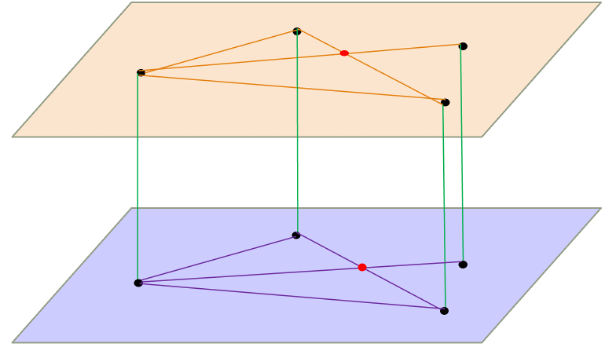
\includegraphics[width=\linewidth]{images/schema_graphe.png}
				\caption{Schéma d'un graphe multimodale}
		\end{minipage}
		\label{fig:reseau_rwanda}
	\end{figure}
	



	
	\subsubsection{Extraction de la composante géante}
	\label{subsubsec:composante_geante}
	
	La première étape pour produire un graphe fonctionnel est de corriger les erreurs topologiques des données géographiques : mettre les données au bon format de géométrie et créer un nœud au niveau du croisement entre deux arêtes.
	
	Une fois fait, on extrait du graphe la composante géante, c'est-à-dire le bloc de route interconnecté le plus grand du graphe. Ce dernier représente environ 96\% des routes du pays présentes sur OSM.
	
	
	\begin{figure}[H]
		\centering
		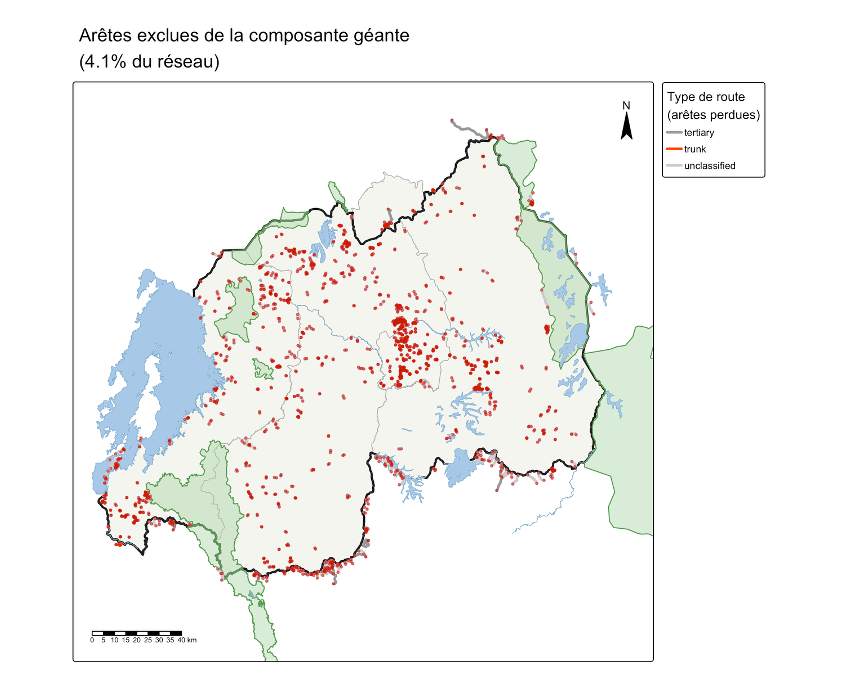
\includegraphics[width=0.6\linewidth]{images/carte_routes_hors_geante.png}
		\caption{Carte des blocs de routes non reliées à la composante géante}
		\label{fig:carte_comp_geante}
	\end{figure}
	
	\begin{figure}[H]
		\centering
		\begin{minipage}{0.48\textwidth}
			\centering
			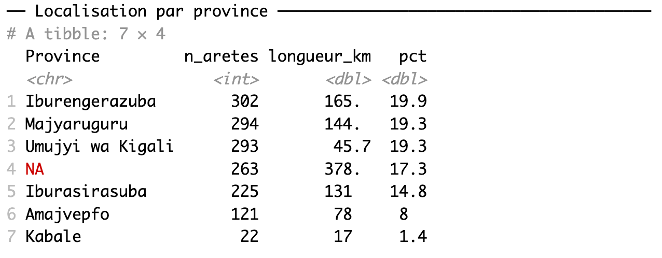
\includegraphics[width=\linewidth]{images/local_routes_hors_geante.png}
			\caption{Localisation des routes non reliées à la composante géante}
			\label{fig:local_routes_hors_geante}
		\end{minipage}
		\hfill
		\begin{minipage}{0.48\textwidth}
			\centering
			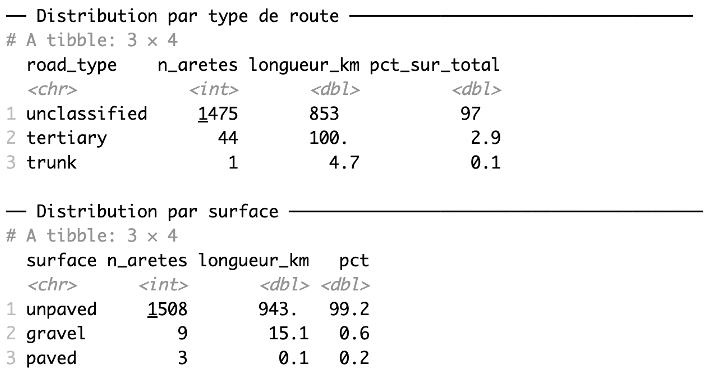
\includegraphics[width=\linewidth]{images/types_routes_hors_geante.png}
			\caption{Types de routes non reliées à la composante géante}
			\label{fig:types_routes_hors_geante}
		\end{minipage}
	\end{figure}
	
	\subsubsection{Intégration des données}
	\label{subsubsec:integ_donnees}
	
	Une fois fait, on ajoute à l'ensemble des arcs, représentant les routes, leurs caractéristiques : 
		
	\begin{itemize}
		\item L'usage du sol : il peut être "zones urbaines" si la droite appartient à une zone tagué comme résidentiel, commercial et retail sur OSM ; "zone industrielle" si elle est taguée ainsi sur OSM ; ou bien "zone rurale" si elle n'a pas de tag
		\item Les pentes : on découpe les routes en bloc de 100m et on attribut à chaque bloc l'altitude tel que définit par le DEM.		
		\item Le coût de transport par tonne transportée sur la route, par mode de transport. Nous précisons dans la section suivante la méthode de calcul de ce coût.
	\end{itemize}
	
	On ajoute ensuite au graphe les points correspondants aux OD du modèle. Pour cela, on ajoute les points définis manuellement ainsi que l'ensemble des villes présentent dans le fichier OSM. Ces points sont snappés sur le noeud du réseau le plus proche afin d'être relié aux routes. Si plusieurs villes sont snappées sur le même point, on ne conserve que la ville avec la plus grande population. On associe ensuite à chaque point son polygone de Voronoï, c'est-à-dire l'ensemble du territoire Rwandais dont aucun autre point du graphe n'est plus proche. L'idée est de supposé que les points du graphe sont représentatifs de l'ensemble du territoire que couvre le polygone de Voronoï.

	Le choix du pavage de Voronoï plutôt que du découpage administratif mérite d'être justifié. Le zonage est en effet le principal levier de biais d'un modèle en quatre étapes : \cite{HolguinVeras2011} montrent que l'erreur de génération croît avec l'hétérogénéité interne des zones, et \cite{Ortuzar2011} rappellent que le découpage doit être défini par rapport au réseau, faute de quoi une part importante des déplacements devient intra-zonale et disparaît du modèle. Or les districts rwandais sont à la fois très hétérogènes (ils mêlent systématiquement centre urbain et versants ruraux) et sans rapport avec la topologie du réseau. Le pavage de Voronoï répond aux deux problèmes : par construction, chaque parcelle du territoire est rattachée au point d'accès au réseau qui lui est effectivement le plus proche, ce qui donne une partition exhaustive, sans recouvrement, et cohérente avec la manière dont les marchandises entrent réellement sur le réseau. Il permet en outre de faire varier la résolution du modèle simplement en ajoutant ou retirant des points OD, sans avoir à redéfinir un zonage.

	On ajoute ensuite à ces polygones leurs caractéristiques :
	\begin{itemize}
	\item La somme de la population tel que présente dans le raster WorldPop ou bien, si elle n'est pas disponible, une partie de la population officielle du districte tel que donnée par NISR au prorata de l'aire du ou des districts que le polygone de Voronoï occupe.
	\item Le RWI moyen. Pour ce faire, on calcul d'abord le rwi moyen brut selon cette formule : 
	\begin{equation}
		\text{RWI}_i = \frac{\sum_i^c \text{rwi}_i \times \omega_i}{\sum_i^c \omega_i }
		\label{eq:rwi brut}
	\end{equation}
	Une fois fait, on procède à une normalisation min-max pour classer entre 0 et 1 l'ensemble des points : 
	\begin{equation}
		p\_rwi_i = \frac{\text{RWI}_i - \min {\text{échantillon}}}{\max{\text{échantillon}}-\min{\text{échantillon}}}
		\label{eq:rwi normalise}
	\end{equation}
	Les NA sont remplacés par la valeur médiane pour ne pas biaisé le rang des points OD.
	\item La somme des emplois par secteur. Chaque polygone reçoit les données de son district au prorata de l'air qu'il y occupe.
	\item La classe géo-sociale. Les polygones sont classés en 10 catégories : par quintile de revenus et s'ils sont urbains ou ruraux. 
	Un polygone est considéré comme urbain si plus de 50\% de sa population vie dans une zone taguée sur OSM comme residential, commercial ou retail. Sinon, le polygone est rural. Si aucun polygone n’est considéré comme urbain, la demande finale des urbains de la SAM est attribuée à la variable dem\_finale\_publique.
	Les quintiles de revenus sont estimés via le $p\_rwi$.	

	\end{itemize}

	
	\subsubsection{Calcul du coût généralisé sans congestion}
	\label{subsubsec:cout_generalise}
	Comme nous l'avons précisé plus haut, chaque arc du graphe reçoit un $\text{coût}_t$. La notion de coût généralisé — une somme pondérée de composantes monétaires et non monétaires, ramenée à une unité commune — est le pivot classique des modèles de transport \cite{Ortuzar2011} ; c'est elle qui permet d'arbitrer entre un itinéraire court mais lent et un itinéraire long mais rapide. Nous l'exprimons par tonne, et non par véhicule, pour deux raisons : c'est l'unité dans laquelle le modèle gravitaire raisonne, et cela évite d'avoir à trancher prématurément la question du taux de remplissage, qui relève d'une décision logistique distincte \cite{HolguinVeras2011}.

	Le choix des composantes retenues découle directement du contexte rwandais (section~\ref{sec:contexte_modele}). Le coût de carburant est modulé par la pente et par la nature de la surface parce que le relief et l'hétérogénéité du revêtement sont les deux caractéristiques dominantes du réseau : sur un réseau dont moins de 5~\% du linéaire est bitumé, une vitesse et une consommation moyennes uniformes reviendraient à supprimer du modèle l'essentiel de ce qui différencie les itinéraires. Le coût du temps est isolé des autres composantes parce qu'il est le seul à être affecté par la congestion, ce qui rend possible la décomposition utilisée à la section~\ref{subsubsec:decompo_cout}. Le facteur urbain, enfin, pénalise les gros véhicules en zone dense, à défaut d'une modélisation explicite du dernier kilomètre.
	
	\begin{equation}
		\text{coût}_t = \frac{ \text{coût}_{\text{fuel}} + (\text{coût}_{\text{usure}} + \text{coût}_{\text{temps}}) \times \text{facteur urbain}}{\text{capacité}_{\text{max tonnes}}}
		\label{eq:cout_t}
	\end{equation}
	
	Où :
	
	\begin{equation}
		\text{coût}_{\text{fuel}} = (\text{conso\_carburant} \times \text{facteur surface}\times (1+\text{pente}\times \frac{\text{facteur pente}}{100})\times \text{distance}_\text{km})\times \text{prix}_\text{fuel}
		\label{eq:cout_fuel}
	\end{equation}
	
	\begin{equation}
		\text{coût}_{\text{usure}} = \text{carburant}_{\text{prix}} \times \text{usure}_{\text{km}}
		\label{eq:cout_usure}
	\end{equation}
	
	\begin{equation}
		\text{coût}_{\text{temps}} = \frac{\text{distance}_{\text{km}}}{\text{vitesse}_{\text{kmh}}} \times \text{prix}_{\text{temps}} 
		\label{eq:cout_temps}
	\end{equation}
	
	Ce coût sera ensuite utilisé comme variable à minimiser par \href{https://fr.wikipedia.org/wiki/Algorithme_de_Dijkstra}{l'algorithme Dijkstra} afin de trouver le plus court chemin entre les différents points du graphe. Chaque point est ainsi relié à l'ensemble des autres par le chemin le plus court. C'est à ce moment que le choix du mode de transport se fait. Les arc de transbordement reçoivent eux uniquement un coût de transbordement définit au début, dans les paramètres. Les couches du réseau par mode de transport étant relié au sein du graphe par ses arêtes de transbordement, il est possible d'aller d'un point A à un point B en passant par plusieurs mode de transport. On suppose donc ici que les entreprises utilisent toujours le mode de transport le moins cher.
	Une fois fait, on a donc une matrice OD où chaque ligne correspond à une pair de points OD à laquelle on associe plusieurs colonne : le coût du chemin optimal, la distance et le temps du parcours, le véhicule de départ et d'arrivé, le nombre de transbordements ainsi que les émissions de polluantes.
	
	\subsection{Production des flux}
	\label{subsec:prod_flux}
	
	Maintenant que nous avons notre graphe multimodale prêt, il faut que nous affection les volumes échangés contenus dans les données de la SAM vers les points OD et que nous les fassions échanger entre eux.
	
	\subsubsection{Affectation locale de la production}
	\label{subsubsec:affectation_prod}
	La production totale par secteurs, telle que définie dans la SAM, est alloué aux différents points OD en proportion du nombre d'emplois de chaque point et de sa richesse relative, utilisée comme proxi de la productivité. L'approximation de la productivité par la richesse relative étant grossière, nous avons choisi de réduire son poids par rapport à celui du nombre d'emplois alloués au point OD.

	Cette manière de procéder est la transposition à l'échelle infranationale de l'approche entrée-sortie multirégionale de \cite{Cascetta2008} : plutôt que d'estimer directement des volumes émis par zone, on part d'un total national comptablement cohérent (ici celui de la SAM 2021) et on le \emph{spatialise} au moyen de clés d'allocation. L'avantage est que la somme des productions locales reste égale, par construction, à la production nationale, ce qui est la condition d'un couplage ultérieur avec un modèle multisectoriel. Le choix de l'emploi comme clé principale répond en outre à la critique de \cite{HolguinVeras2011} sur les taux de génération constants : c'est bien une variable d'activité sectorielle, et non un taux uniforme appliqué à la population ou à la surface, qui détermine les tonnes émises. Le pondérateur $\alpha = 0{,}7$ traduit enfin un arbitrage explicite : il conserve un effet de productivité différenciée entre zones riches et zones pauvres, tout en limitant l'influence d'un indicateur — le RWI — qui mesure la richesse des ménages et non celle de l'appareil productif \cite{Chi2022}. Sa valeur est reprise dans les tests de sensibilité (section~\ref{sec:sensibilite}).
	
	\begin{equation}
		x_{i,s} = \text{prod\_totale}_s \times w_{i,s}
		\label{eq:prod_i}
	\end{equation}
	
	Où :
	
	$x_{i,s}$ = production du secteur s de l’entrepôt i
	

	$w_{i,s} = \alpha \times \frac{\text{emploi}_{i,s}}{\sum_i \text{emploi}_{i,s}} + (1 - \alpha) \times \frac{\text{p\_rwi}_{i}}{\sum_i \text{p\_rwi}_{i}}$, avec $\alpha$ = 0,7

	

	
	\subsubsection{Affectation locale de la consommation}
	\label{subsubsec:affectation_conso}
	
	La demande totale utilisées ensuite dans le modèle gravitaire est la somme des différentes composantes de la demande que comprend la SAM, c'est-à-dire les consommation intermédiaire et les consommations finales.
	
	\begin{equation}
		d_{i,s} = d\_\text{inter}_{i,s} + d\_\text{finale}_{i,s} 
		\label{eq:conso}
	\end{equation}\\
	
	Les consommations intermédiaires sont dérivées, très classiquement, du produit de la matrice des coefficients techniques et du vecteur de la production totale de l'entrepôt i calculé via l'équation \ref{eq:prod_i}. N'ayant pas d'information concernant l'hétérogénéité des systèmes techniques par point OD, nous avons fait le choix d'utiliser uniformément la matrice nationale des coefficients techniques. Il s'agit de l'hypothèse standard des modèles entrée-sortie régionalisés lorsque les tables régionales n'existent pas \cite{Miller2009} : on suppose que la technologie de production d'un secteur est nationale, et que seule sa localisation varie. Elle est ici d'autant plus tenable que le Rwanda est un petit territoire à structure productive peu diversifiée (section~\ref{sec:structure_productive}), mais elle reste une limite reconnue du travail.

	Le fait de dériver la demande intermédiaire de la production locale plutôt que de l'estimer indépendamment est ce qui donne au modèle sa cohérence : chaque tonne produite quelque part engendre mécaniquement une demande d'intrants qui devra être satisfaite ailleurs, et c'est cet écart local entre ce qui est produit et ce qui est consommé qui alimente le modèle gravitaire (section~\ref{subsubsec:decompo_comex}). Sans ce bouclage entrée-sortie, les marges du modèle gravitaire seraient arbitraires.
	
	\begin{equation}
		d\_\text{inter}_{i,s} = \sum_r A_{r,s} \times x_{i,r}
		\label{eq:conso_inter}
	\end{equation}
	
	Avec : 
	
	$d\_\text{inter}_{i,s}$ = demande des consommations intermédiaires du secteur s de l'entrepôt i.
	
	$A_{r,s}$ = quantité de biens du secteur s consommée pour produire une unité de bien du secteur r. \\ 

	La demande finale elle se décompose en deux composantes. D'une part, la demande finale des ménages et d'autre part les dépenses publiques et dépenses d'investissement. 
	
	\begin{equation}
		d\_\text{finale}_{i,s} = d\_\text{finale\_publique}_{i,s} + d\_\text{finale\_ménage}_{i,s} 
		\label{eq:conso_finale}
	\end{equation}\\
	
	La demande finale des ménages du secteur s de l'entrepôt i ($d\_\text{finale\_ménage}_{i,s}$) est calculée en proportion de la population via la formule suivante :
	
	\begin{equation}
		d\_\text{finale\_ménage}_{i,s} = \sum_c F_{c,s}\times \frac{\text{pop}_{i,c}}{\sum_j \text{pop}_{j,c}}
		\label{eq:conso_finale_menage}
	\end{equation}\\
	
	Avec :
	
	$\text{pop}_{j,c}$ = la population de l'entrepôt i de la classe géo-sociale c telle que définie dans la section \ref{subsubsec:integ_donnees}.
	
	$F_{c,s}$ = demande finale nationale du secteur s et de la classe géo-sociale c.\\

	
	Finalement, on complète la demande finale par celle relevant de la consommation publique et des l'investissement public et privé. Les imports et exports sont traité à part. 
	
	\begin{equation}
 	d\_\text{finale\_publique}_{i,s} = F\_\text{publique}_s\times \frac{z_i}{\sum_j z_j}
 		\label{eq:conso_finale_publique}
	\end{equation}
	
	Avec :
	
	$F\_\text{publique}_s$ = consommation publique (gov) et investissement (s-i) dans le secteur s à l'échelle nationale
	
	$z_i = \text{pop}_i \times (p\_rwi_i + \epsilon)$ = poids de l'entrepôt i dans la demande finale nationale. 

	
	\subsubsection{Création d'une couche Rest of World (RoW)}
	\label{subsubsec:RoW}
	
	Afin de maintenir l'équilibre emplois-ressources de la SAM, nous avons intégré les flux en provenance et à destination du reste du monde. Pour ce faire, nous avons ajouté une couche géographique RoW composée des 4 pays frontaliers : Ouganda, Tanzanie, RDC et Burundi.
	
	Les importations et exportations totales du Rwanda définies dans la SAM sont réparties par pays en fonction d'une clé de répartition exogène générée par le LLM Claude. 
	
	\subsubsection{Modèle gravitaire doublement contraint}
	\label{subsubsec:gravitaire}
	
	C'est le c\oe ur du modèle. L'idée est que deux points OD ont d'autant plus de chance d'échanger ensemble d'un bien s que l'un en produit beaucoup, l'autre en demande beaucoup et que le coût de transport entre les deux points est faible. Pour cela, on procède par itération via l'algorithme de Furness.

	Le recours à un modèle gravitaire \emph{doublement} contraint — plutôt qu'à un modèle simplement contraint ou libre — se justifie par la nature de l'information dont nous disposons. Les sections précédentes fournissent, pour chaque point OD et chaque secteur, un surplus d'offre et un déficit de demande comptablement cohérents avec la SAM ; en revanche, aucune matrice origine-destination de fret n'est observée au Rwanda. Or c'est exactement la situation pour laquelle le modèle doublement contraint a été conçu : \cite{Wilson1967} montre qu'il produit la distribution la plus probable — au sens de l'entropie maximale — parmi toutes celles compatibles avec les deux marges et avec un budget de coût de transport, et \cite{Cai2021} établit que sous ces conditions les flux inconnus peuvent être reconstruits exactement, avec beaucoup moins de données que ne le suppose généralement la littérature. Imposer les deux marges garantit de surcroît que le modèle ne peut ni créer ni détruire de matière : la conservation comptable héritée de la SAM est préservée jusqu'au niveau des flux physiques, condition nécessaire au couplage macroéconomique visé.

	Le prix de cette approche est qu'elle est agnostique quant au comportement des agents : elle ne dit pas \emph{pourquoi} deux zones échangent, seulement que la distribution retenue est la moins informative compatible avec les contraintes. C'est une limite assumée, cohérente avec le positionnement du travail en \emph{proof of concept}, mais qui la distingue nettement des approches micro-fondées de type ABM ou ADA évoquées aux sections~\ref{subsec:ADA} et~\ref{subsec:ABM}.
	
	\begin{equation}
		T_{ij}^s = A_{i,s} \times B_{j,s} \times O_{i,s} \times  \left( \frac{\text{tonnes}}{\text{Milliard RWF}} \right)_s \times D_{j,s}  \times \left( \frac{\text{tonnes}}{\text{Milliard RWF}} \right)_s \times \text{Friction}_{i,j}^s
		\label{eq:gravitaire}
	\end{equation}
	
	Où :
	
	\begin{itemize}
		\item $T_{ij}^s$ = flux du secteur $s$ de l'entrepôt $i$ vers le $j$ (Tonnes)
		\item $\text{Friction}_{i,j}^s$ = mesure du découragement des échanges du secteur $s$ entre $i$ et $j$ en raison des coûts de transport
		\item $O_{i,s}$ = exportations du secteur $s$ de l'entrepôt $i$ (Milliards de RWF)
		\item $D_{j,s}$ = importations du secteur $s$ de l'entrepôt $j$ (Milliards de RWF)
		\item $A_{i,s}$, $B_{j,s}$ = facteurs d'équilibrage calculés par l'algorithme de Furness (IPF)
	\end{itemize}
	
	\subsubsection{Fonction de friction}
	\label{subsubsec:friction}
	
	La fonction de friction à pour objet de capter la sensibilité des échanges aux coûts de transport.

	Trois choix de spécification méritent d'être explicités. Premièrement, l'argument de la fonction est un coût généralisé en USD par tonne, et non une distance : c'est ce qui permet au relief, à l'état du revêtement et aux ruptures de charge d'agir sur la distribution des flux, et donc à un choc localisé sur le réseau de se traduire par une réallocation des échanges. Deuxièmement, la forme retenue est une puissance négative plutôt qu'une exponentielle. \cite{deJong2004} et \cite{Ortuzar2011} rappellent que les deux formes sont d'usage courant et que le choix se tranche normalement par calibration sur des flux observés ; en l'absence de telles données, nous retenons la forme puissance parce qu'elle décroît plus lentement en queue et évite ainsi d'annuler mécaniquement les échanges longue distance — ce qui, sur un territoire de la taille du Rwanda et avec un commerce extérieur passant par des corridors de plus de 1~500~km (section~\ref{sec:tout_routier}), serait une erreur de spécification. Troisièmement, le coût fixe de manutention est ajouté \emph{à l'intérieur} de la parenthèse, avant l'exponentiation : il joue donc comme un plancher de coût, ce qui empêche la friction de diverger pour les paires très proches et reproduit le fait, documenté par \cite{Tavasszy2012}, qu'une part substantielle du coût logistique est indépendante de la distance parcourue.

	Le paramètre $\beta_s$ est le paramètre le plus déterminant et le moins bien identifié du modèle : faute de flux observés, il est produit par dire d'expert (section~\ref{subsubsec:donnees_fictives}). C'est la raison pour laquelle il fait l'objet d'un test de sensibilité dédié (section~\ref{subsec:parametre_friction}).
	
\begin{equation}
		\text{Friction}_{i,j}^s = \left[ c_{ij} + c_{p,j,s} + c_{\text{fixe}} \times \left( \frac{\text{tonnes}}{\text{Milliard RWF}} \right)_s \right]^{-\beta}
		\label{eq:friction}
\end{equation}
	
	Où :
	
	\begin{itemize}
		\item $c_{ij}$ = coût de transport (USD / tonne) entre $i$ et $j$ issue de la matrice OD
		\item $c_{p,j,s} = \min_b[\text{coût\_frontière}_{p,s} + c_{b,j}]$ = coût de transport entre le pays $p$ et l'entrepôt $j$ via le poste à frontière $b$
		\item $c_{\text{fixe}}$ = coût fixe de manutention (chargement + déchargement) (USD / tonne)
		\item $\beta_s$ = paramètres de friction (sensibilité) par secteur
	\end{itemize}
	
	\subsubsection{Algorithme de Furness (IPF)}
	\label{subsubsec:furness}
	
	\textbf{Initialisation} On part de la matrice non contrainte, qui respecte
	la structure de friction mais aucune des deux marges :
	
	\begin{equation}
		T_{i,j}^s = O_{i,s} \times D_{j,s} \times \text{Friction}_{i,j}^s
	\end{equation}\\
	Avec $T_{ii}^{s} = 0$ : les échanges intra-zones ne sont pas pris en compte
	
	\textbf{Boucle :} À l'itération $k$, on alterne deux rééquilibrages.
	
	1) Équilibrage des lignes $i$ :
	
	\begin{equation}
		T_{i,j}^s \leftarrow T_{i,j}^s \times A_{i,s,k}
	\end{equation}
	
	Où $A_{i,s,k} = \frac{O_{i,s}}{\sum_j T_{i,j}^s}$
	
	L'objectif est que $A_{i,s,k} \to 1 \iff O_{i,s} = \sum_j T_{i,j}^s$. L'ensemble flux sortant du point OD i doit être égale au surplus de production de ce dernier tel que définit dans la section \ref{subsubsec:decompo_comex} ci-dessous. C'est la première contrainte.\\
	
	2) Équilibrage des colonnes $j$ :
	
	\begin{equation}
		T_{i,j}^s \leftarrow  T_{i,j}^s \times B_{j,s,k} 
	\end{equation}
	
	Où $B_{j,s,k} = \frac{D_{j,s}}{\sum_i T_{i,j}^s}$
	
	L'objectif est que $B_{i,s,k} \to 1 \iff D_{i,s} = \sum_j T_{i,j}^s$. C'est la deuxième contrainte. L'ensemble flux entrant du point OD i doit être égale au déficit de production de ce dernier tel que définit dans la section \ref{subsubsec:decompo_comex} ci-dessous.\\
	
	L'algorithme itère jusqu'à ce que la différence entre les flux sortants/entrants et l'offre/demande soit inférieure à un seuil de tolérance, c'est-à-dire que $A_{i,s}$ et $B_{j,s}$ tendent assez vers 1.
	
	\textbf{Lien avec le modèle doublement contraint.} Les facteurs
	\emph{cumulés} sur l'ensemble des itérations,
	%
	\begin{equation}
		A_i^s = \prod_k a_i^{s,(k)},
		\qquad
		B_j^s = \prod_k b_j^{s,(k)},
	\end{equation}
	%
	sont les facteurs d'équilibrage du modèle de \cite{Wilson1967}, et la
	solution s'écrit sous forme fermée
	$T_{ij}^s = A_i^s B_j^s O_i^s D_j^s (C_{ij}^s)^{-\beta_s}$.

	Le choix de cet algorithme plutôt que d'une résolution directe tient à trois propriétés. D'abord, il converge vers l'unique solution du programme de maximisation d'entropie sous contraintes de marges dès lors que le problème est faisable, et cette solution est indépendante du point de départ : les facteurs cumulés $A_i^s$ et $B_j^s$ ne sont rien d'autre que les multiplicateurs de Lagrange des contraintes \cite{Wilson1967}. Ensuite, il est peu coûteux — chaque itération se réduit à deux normalisations de matrice — ce qui compte ici, puisqu'il est exécuté séparément pour chaque secteur et pour chacune des trois jambes du commerce (section~\ref{subsubsec:decompo_comex}), et réexécuté à chaque scénario de rupture. Enfin, il est identique à l'algorithme RAS de la comptabilité entrée-sortie, ce qui assure la continuité méthodologique avec l'origine des données : \cite{Cai2021} montre précisément que les principales procédures d'estimation de matrices de commerce interrégional convergent vers ce même cadre.

	Sa contrepartie est une exigence de faisabilité stricte : l'algorithme ne converge que si les marges lignes et colonnes ont la même somme et si le support de la matrice de friction le permet. C'est ce point qui a rendu nécessaire la décomposition en trois jambes exposée ci-dessous.
	
	
	\subsubsection{Décomposition entre commerce domestique et extérieur}
	\label{subsubsec:decompo_comex}
	
	L'algorithme de Furness est appliqué 3 fois : pour les échanges domestiques, pour les exportations et pour les importations.
	
	Dans le cas des :
	
	\begin{itemize}
		\item Échanges domestiques :
		\begin{itemize}
			\item $O_{i,s} = \max (x_{i,s}(1-\tau_{E,s})-d_{i,s}(1-\tau_{M,s});0)$\\
									= surplus d'offre domestique par rapport à la demande du secteur s de l'entrepôt i.
			\item $D_{j,s} = \max (0; d_{j,s}(1-\tau_{M,s})-x_{j,s}(1-\tau_{E,s}))$\\
									= idem pour le déficit.
		\end{itemize}
		\item Exports : 
		\begin{itemize}
			\item $O_{i,s} = \tau_{E,s} \times x_{i,s}$ = part de la production du secteur s de l'entrepôt i qui est exportée.
			\item $D_{j,s} = EX_{j,s}$ = total des exportations du secteur s vers le pays j.
		\end{itemize}
		\item Imports :
		\begin{itemize}
			\item $O_{i,s} = IM_{s,i}$ = total des importations du secteur s depuis le pays i.
			\item $D_{j,s} = \tau_{M,s}\times d_{i,s}$ = part de la demande du secteur s de l'entrepôt j qui est importée.
		\end{itemize}
	\end{itemize}
	
	
	
	Avec : $\tau_{E,s} = \frac{EX_s}{\text{prod\_totale}_s}$ et $\tau_{M,s}=\frac{IM_s}{\sum_i d_i}$
	
	\subsection{Affectation du fret}
	\label{subsec:affectation_fret}
	
	\subsubsection{Décomposition coût sans congestion}
	\label{subsubsec:decompo_cout}
	
	Le coût\_tkm précédemment calculé = coût sans congestion qu'on multiplie par les km de la route $i$ pour avoir $\text{coût}_{t,i}$.
	
	On le décompose entre sa partie temps et hors temps :
	
	\begin{equation}
		\text{coût}_{v,i} = \text{coût\_hors\_temps}_{v,i} + \text{coût\_temps}_{v,i}
	\end{equation}
	
	\begin{equation}
		\text{coût\_temps}_{v,i} = \text{temps}_{v,i} \times \frac{\text{valeur\_temps}_v}{\text{distance\_parcourue}_v}
	\end{equation}
	
	Où :
	
	\begin{itemize}
		\item $\text{temps}_{v,i}$ = temps de transport d'un véhicule $v$ sur la route $i$ en heure
		\item $\text{temps\_valeur}_v$ = valeur exogène d'une heure de transport du véhicule $v$
	\end{itemize}
	
	\subsubsection{Fonction de congestion BPR (Bureau of Public Roads)}
	\label{subsubsec:BPR}
	
	
	La fonction de congestion du \cite{BPR1964} est l'approche standard pour modéliser l'impact de la congestion sur les temps de trajet. Elle est la fonction débit-retard la plus employée depuis soixante ans, pour trois raisons : elle ne requiert que deux paramètres, elle est continue et strictement croissante — donc convexe en flux, ce qui garantit l'existence et l'unicité de l'équilibre de \cite{Wardrop1952} au sens de \cite{Beckmann1956} — et elle est peu coûteuse à évaluer, ce qui importe puisqu'elle est recalculée sur chaque arc à chaque itération.
	
	\begin{equation}
		\text{facteur\_BPR}_{i,n} = \left[ 1 + \alpha \times \left( \frac{\text{PCU}_{i,n}}{\text{C}_i} \right)^\beta \right]
	\end{equation}
	
	Où :
	
	\begin{itemize}
		\item $\text{C}_i$ = capacité de PCU/jour sans congestions sur la route $i$
		\item $\text{PCU}_{i,n}$ = PCU/jour effectif sur la route $i$ à l'itération $n$
		\item $\alpha$ et $\beta$ = paramètres = 0.15 et 4, valeurs de référence du \cite{BPR1964}, toujours standard dans la littérature
	\end{itemize}

	\vspace{1em}

	L'objectif est que le surcoût en termes de temps de rajouter une voiture soit très faible tant que $\text{PCU}_i < \text{C}_i$ et augmente très rapidement ensuite. Deux précisions sur l'usage que nous en faisons. D'une part, seule la composante temps du coût généralisé est multipliée par le facteur BPR (section~\ref{subsubsec:decompo_cout}) : la congestion allonge les durées, elle ne modifie ni la pente ni la consommation à vitesse donnée. D'autre part, nous conservons les valeurs standards $\alpha$ et $\beta$ faute de comptages routiers permettant de les recalibrer sur le réseau rwandais ; la capacité $C_i$ étant elle-même produite par dire d'expert, les niveaux absolus de congestion obtenus doivent être lus comme indicatifs, et c'est la \emph{hiérarchie} des arcs congestionnés qui est exploitable.
	
	\subsubsection{Flux PCU journalier par route}
	\label{subsubsec:PCU}
	
	On calcule pour chaque route le flux d'équivalents véhicules individuels par jour (PCU) :
	
	\begin{equation}
		\forall n \in \{\text{itérations}\},
		 \quad \text{PCU}_{i,n}^* = \frac{\text{tonnes}_{i,n}^{s,*}}{\text{taux\_chargement} \times \text{capacité\_max}_v} \times \frac{\text{facteur\_PCU}_v}{ \text{jours\_trafic}_{\text{an}}}
	\end{equation}
	
	Avec : 
	
	$\text{facteur\_PCU}_v$ = équivalent véhicule individuel du véhicule v
	
	$\text{capacité\_max}_v$ = capacité maximale de chargement du véhicule v
	
	$\text{taux\_chargement}$ = proportion de la capacité maximale
	
	$\text{jours\_trafic}_{\text{an}}$ = nombre de jours ouvrables de frafic fret par an
	
	
	\subsubsection{Méthode des moyennes successives (MSA)}
	\label{subsubsec:MSA}

	Le couple flux-coût est un point fixe : les flux dépendent des coûts par le plus court chemin, et les coûts dépendent des flux par la fonction BPR. On le résout par la méthode des moyennes successives (MSA) décrite par \cite{Sheffi1985}, qui consiste à moyenner la solution courante avec l'affectation « tout ou rien » obtenue à l'itération en cours, avec un poids décroissant en $1/n$. Ce choix se justifie par sa robustesse : contrairement à une mise à jour brutale des flux, qui fait osciller la solution entre itinéraires concurrents sans converger, la décroissance du pas garantit la convergence vers l'équilibre de \cite{Wardrop1952} et ne demande ni calcul de dérivée ni recherche linéaire. Sa lenteur asymptotique, principal reproche qui lui est fait, est ici sans conséquence : le critère d'arrêt porte sur la stabilité relative des flux PCU, atteinte en un nombre modéré d'itérations sur un réseau de cette taille.

	On procède par itérations.
	
	Itération $n$ :
	
	\begin{equation}
		\text{coût}_{v,i,n} = \text{coût\_hors\_temps}_{v,i} + \text{coût\_temps}_{v,i} \times \text{facteur\_BPR}_{i,n}
	\end{equation}
	
	\begin{equation}
		\text{temps}_{t,i,n} = \text{temps}_{t,i,n-1} \times \text{facteur\_BPR}_{i,n}
	\end{equation}
	
	\begin{equation}
		\text{tonnes}_{t,n}^{s,*} = \text{tonnes}_{t,n-1}^{s,*} + \frac{1}{n} \times (\text{tonnes}_{t,n}^s - \text{tonnes}_{t,n-1}^{s,*})
	\end{equation}
	
	Où :
	

	 $\text{tonnes}_{t,n}^{s,*}$ = flux d'équilibre de marchandises du secteur $s$ sur l'arête $i$ après l'itération $n$
	 
	 $\text{flux}_{t,n}^s$ = flux courant de marchandises du secteur $s$ sur l'arête $i$ lors de l'itération $n$\\

	
	On s'arrête lorsque :
	
	\begin{equation}
		\frac{\sum_i |\text{PCU}_{i,n}^* - \text{PCU}_{i,n-1}^*|}{\sum_i \text{PCU}_{i,n}^*} < \text{seuil}
	\end{equation}
	
	\subsubsection{Coût logistique total pour la comptabilité}
	\label{subsubsec:compta_logistiq}
	
	La modélisation du coût logistique total intègre les approches de \cite{Baumol1970} sur les modèles de transport de fret et \cite{Tavasszy2012} sur l'intégration de la logistique dans les modèles de demande de transport de fret.\\

	Cette comptabilité répond à une limite reconnue des modèles en quatre étapes : le choix d'itinéraire y est fait sur le seul coût de déplacement, alors que la décision réelle du chargeur porte sur un coût logistique total incluant l'immobilisation de capital en stock et en transit. \cite{Baumol1970} en donnent la formulation fondatrice en transposant le modèle de lot économique (EOQ) au transport de fret : la taille optimale des envois résulte de l'arbitrage entre coût fixe par envoi et coût de détention du stock, et le temps de transport entre dans le coût par le stock en transit. \cite{Combes2012} en fournit la validation empirique sur données d'enquête chargeurs françaises, et \cite{Tavasszy2012} montrent, dans leur revue, que l'omission de ces composantes conduit à sous-estimer systématiquement la sensibilité du fret à la fiabilité et à la durée des trajets.

	Nous retenons cette formulation comme \emph{comptabilité ex post} et non comme critère d'optimisation : le choix du chemin et du véhicule reste fait sur le coût généralisé de la section~\ref{subsubsec:cout_generalise}, et le coût logistique total est reconstruit ensuite, jambe par jambe, sur les flux d'équilibre. Ce découplage est un choix assumé de simplicité — il évite une boucle d'optimisation supplémentaire dont les paramètres (valeur à la tonne, taux de détention) sont ici issus de dire d'expert — mais il constitue une limite : le modèle ne peut pas représenter un report d'itinéraire motivé par la seule réduction du stock en transit.
	
	Coût Logistique Total = coût fixe de transport + coût variable du transport + coût de stockage + coût de stock en transite
	
	\begin{equation}
		\begin{aligned}
			\text{CLT}_{s,v,i,j} = {}& \frac{T_{i,j}^s}{\text{q}_{i,j,v}} \times K_v \\
			& + T_{i,j}^s \times \left( \sum_i \text{coût}\_t_{v,i,n} \right) \\
			& + \frac{\text{taille\_envoi}_{i,j,v}}{2} \times V_s \times r \\
			& + T_{i,j}^s \times \tau_v \times V_s \times r
		\end{aligned}
	\end{equation}
	
	Où :
	

	$\tau_v = \frac{ \sum_k\text{temps}_{v,k}}{\text{heure\_année}} $ = temps de trajet entre $i$ et $j$ via la partie du trajet effectué avec le véhicule v en proportion de l'année
	
	$\text{q}_{i,j,v}$ = taille optimale des envois entre $i$ et $j$ via la partie du trajet effectuée avec le véhicule v
	
	$K_v$ = coût d'embarquement + débarquement
	
	$V_s$ = valeur d'une tonne de marchandise du secteur $s$
	
	$r$ = taux de détention du stock = coût annuel de garder une unité de valeur en stock = taux d'intérêt + coût stockage + assurance + obsolescence

	
	\subsection{Modélisation d'un choc}
	\label{subsec:choc}

	C'est ici que se justifie a posteriori l'ensemble des choix précédents. Représenter explicitement le réseau arc par arc n'a d'intérêt que si l'on veut que la \emph{localisation} du choc, et non seulement son ampleur, détermine ses conséquences économiques — ce qui est précisément l'angle mort des modèles SCGE discutés à la section~\ref{subsec:SCGE}. La méthode retenue relève de l'analyse de vulnérabilité des réseaux telle que formalisée par \cite{Jenelius2015} : on dégrade le réseau, on recalcule les plus courts chemins, et l'on mesure l'impact par l'écart de coût généralisé entre le réseau nominal et le réseau dégradé. \cite{Koks2019} en donnent l'application à l'échelle globale pour les aléas multiples affectant routes et voies ferrées, et \cite{Colon2021} montrent, sur le cas de la Tanzanie, que la criticité d'un tronçon dépend beaucoup moins du trafic qu'il porte que de l'absence d'itinéraire de report — résultat qui motive directement notre choix de mesurer la criticité par le surcoût induit plutôt que par le volume transporté. Le constat du chapitre~\ref{chap:contexte}, selon lequel près de 60~\% des dommages des inondations de mai 2023 ont porté sur le secteur des transports \cite{MINECOFIN2023}, confirme la pertinence de cette entrée pour le Rwanda.

	\subsubsection{Génération de scénarios de rupture}
	\label{subsubsec:scenarios}

	3 modes :
	
	\begin{enumerate}
		\item \textbf{Mode Manuel} : liste d'osm\_id des routes que l'on veut perturber
		\item \textbf{Mode Buffer zone} : toutes les routes dans un rayon autour d'un point donné manuellement sont considérées comme à risque
		\item \textbf{Mode Raster risque} : les routes sont considérées comme en zone à risque si la variable physique est supérieure à un seuil défini (ex: $>$ x millimètres de précipitation)
	\end{enumerate}
	
	Pour les modes Buffer et Raster : on choisit la proportion des routes en zones à risques effectivement inondées. Les routes effectivement inondées seront ensuite générées aléatoirement.
	
	Une fois les routes affectées identifiées, on reconstruit le graphe multi-modal en leur attribuant un coût infini. Ensuite, on recalcule les itinéraires OD optimaux sur ce réseau dégradé.
	
	\subsubsection{Impacts}
	
	\begin{itemize}
		\item Surcoût absolu : coût\_dégradé -- coût\_origine
		\item Surcoût relatif : \% de variation du dégradé par rapport à l'origine
	\end{itemize}
	
	3 types d'impact possibles :
	
	\begin{enumerate}
		\item Déconnecté : plus aucun chemin possible
		\item Surcoût / augmentation de la distance
		\item Inchangé : le chemin optimal ne passe pas par la zone perturbée
	\end{enumerate}
	
	Si la distance augmente, on a aussi une augmentation des émissions.
	
	\subsubsection{Analyse de criticité}
	\label{subsubsec:criticite}

	L'analyse de scénarios répond à la question « que se passe-t-il si cette zone est inondée ? ». L'analyse de criticité répond à la question inverse, indépendante de tout scénario : quelles arêtes du réseau sont les plus coûteuses à perdre ? Elle suit la méthode de suppression d'arc de \cite{Jenelius2015}, où l'importance d'un lien se mesure par l'augmentation du coût total de déplacement induite par sa suppression. Le filtrage préalable aux arêtes les plus chargées et aux paires échangeant des volumes significatifs est une concession au coût de calcul — le problème complet est quadratique en nombre de paires — et introduit un biais qu'il faut signaler : une arête peu chargée mais sans substitut peut être plus critique qu'une arête très chargée doublée par un itinéraire équivalent, ce qui est exactement le phénomène mis en évidence par \cite{Colon2021}.

	\begin{enumerate}
		\item Filtre des arêtes candidates : les arêtes du top $N_{\text{TOP\_ARETES\_CRITIQUES}}$ (=50) des volumes transportés
		\item Passage à coût infini de ces arêtes candidates une par une
		\item Calcul à nouveau de Dijkstra avec comme poids les coûts post-congestion de l'affectation initiale pour les paires qui échangent des volumes supérieurs à $\text{SEUIL\_PAIRES\_CRITICITE}$ (=100t) pour trouver le nouveau chemin le plus court lorsqu'une arête est « supprimée »
		\item Calcul du surcoût servant à classer les arêtes par ordre de criticité
	\end{enumerate}
	
	\newpage
	
	\chapter{Résultats et tests de sensibilité}
	
	\section{Scénario de référence}
	\label{sec:ref}
	
	\subsection{Génération Offre-Demande}
	\label{subsec:OD}
	
	[À développer avec résultats et visualisations]
	
	\subsection{Affectation du fret}
	\label{subsec:affectation_ref}
	
	[À développer avec résultats et visualisations]
	
	\section{Scénarios d'inondations}
	\label{sec:scenario}
	
	La modélisation des impacts des inondations sur les réseaux de transport s'appuie sur les travaux de \cite{Botzen2019} et \cite{Otto2017} qui analysent les impacts économiques des catastrophes naturelles et la propagation des chocs dans les chaînes d'approvisionnement.
	
	\subsection{Impacts}
	\label{subsec:impacts}
	
	[À développer avec résultats et visualisations]
	
	\subsection{Analyse de vulnérabilité}
	\label{subsec:vulneralibilite}
	
	[À développer avec résultats et visualisations]
	
	\section{Tests de sensibilité}
	\label{sec:sensibilite}
	
	Pour l'ensemble des paramètres étudiés, nous avons fait varier leur valeur de $\pm 5\%$.
	
	\subsection{Paramètres de la fonction de friction}
	\label{subsec:parametre_friction}
	
	[À développer avec résultats]
	
	\subsection{Homogénéité de l'exposition au commerce internationale}
	
	
	[À développer avec résultats]
	
	\subsection{Valeur du temps}
	
	[À développer avec résultats]
	
	\subsection{Valeurs des taux de conversion monnaie-tonne}
	
	[À développer avec résultats]
	
	\newpage
	
	\chapter{Discussion}
	
	Les modèles entrée-sortie pour l'évaluation des impacts des catastrophes naturelles \cite{Miller2009, Leontief1936, Okuyama2007} constituent le cadre théorique fondamental de cette analyse. Les travaux récents de \cite{Carvalho2021} et \cite{Inoue2019} sur la propagation des chocs dans les chaînes d'approvisionnement ont également fortement influencé la conception de ce modèle.
	
	\section{Limites du travail}
	
	Le travail présenté comporte un certain nombre de limitations qui méritent d'être mentionnées :
	
	\begin{itemize}
		\item Les routes sont considérées comme étant à double sens (pour réduire le nombre de calculs)
		\item Tous les entrepôts ne sont pas des points OD. Pas possible de faire un changement modal à l'entrée d'une ville par exemple
		\item Hypothèse d'homogénéité des biens et services au sein des secteurs (EX d'un entrepôt $i$ = $O_i$ -- $D_i$)
		\item Hypothèse que la matrice des coefficients techniques $(A)$ est identique entre les différents entrepôts
		\item Hypothèse d'exposition uniforme de tous les entrepôts au commerce extérieur
		\item Hypothèse d'uniformité du prix du temps
		\item Pas de modélisation du dernier km
		\item Pas d'effet du secteur sur le choix modal et le chemin optimal
		\item Le choix modal et le chemin optimal ne tiennent pas compte de l'ensemble des coûts logistiques
		\item La répartition des flux est déterministe et pas probabiliste, ce qui risque de concentrer artificiellement les flux sur certaines routes
		\item RWI représente la richesse des ménages, pas l'activité productive locale
		\item Le transbordement n'a pas de temps associé
		\item Pas de rétroactions de l'effet de la congestion sur les volumes échangés par paire d'entrepôts
	\end{itemize}
	
	\section{Extensions futures et recommandations}
	
	[À développer]
	
	\newpage
	
	\chapter{Conclusion}
	
	[À développer]
	
	\newpage
	
	\chapter*{Bibliographie}
	\addcontentsline{toc}{chapter}{Bibliographie}
	
	\nocite{Barrot2016, BenAkiva2013, Combes2012, deJong2013, Dietzenbacher2013,
		Felbermayr2014, Gabaix2011, Guan2020, Guilbault2009, Hallegatte2013,
		Hallegatte2017, Henriet2012, Hsiang2010, Koks2016, Liedtke2009,
		Lucas1977, Maoh2008, McFadden1974, Okuyama2014, Ortuzar2011,
		Pichler2022, Poledna2018, Rose2007, Rose2005, Rozenberg2019,
		Santos2004, Tavasszy2014, Tsuchiya2007}
		
			% Forcer l'affichage des références non encore citées, à la fin
		\printbibliography[heading=none]
		
		\newpage
		
		\chapter{Annexes}
		
		\subsubsection{Quelques caractéristiques techniques du modèle}
		Le projet a été développé via plusieurs scripts RStudio interdépendants. L'ensemble de ces scripts ainsi que l'ensemble des cartes, graphiques et certaines données sont accessibles librement via le \href{https://github.com/GEMMES-AFD/Transport}{GitHub de l'AFD}
		
	
\end{document}